\section{Navbox}
At the beginning of the semester the \gls{navbox} interface, describe in detail in Chapter 4 and 5 of the \preproject, worked properly.
The only complication was that \gls{apikey} to \gls{kartverket}s CPOS service had expoered, which was resolved by contacting them and asking for a new key with a longer expiration date.

Months later, when I started creating a page for the \gls{navbox} in the \srgui the \gls{navbox} interface had stopped working as no data was received from the \gls{navbox}.
The \gls{navbox} had been stored unused in a drawer since the verification.
Thre potential culprits were identified.

\subsection{Potential cause 1: \jx software}
The first potential culprit is that the \gls{spi} driver, the \gls{spi} \py interface or the \gls{gpio} interface stopped working when the \jx was flashed with the new \gls{os}.

\subsection{Potential cause 2: damage from exessive input voltage}
The \gls{pico} might have been damaged by exessive input voltage from the \gls{stim}.
Revisiting the \gls{navbox} scematics, Figure 27 of the \preproject, and measuring voltages with a multimeter revealed that the \gls{tov} signal from the \gls{stim} was clost to $5V$.
This is not supported by the \gls{gpio} pins on the \gls{pico} \cite[17]{PicoDatasheet}.
It is however not likely that this has caused damage as the \gls{pico} normally can tolerate $5V$ without getting damaged \cite{aryavoronovaRP20405VLogic2023}
Still, the voltage of the digital output signals on the \gls{stim} was configured to $3.3V$ according to Table 12-1 in the \gls{stim} datasheet to make sure this is not an issue in the future \cite[118]{safranSTIM300Datasheet}

\subsection{Potential cause 3: damage to hardware}
A third option is that one ore more wire or connections have been damaged.
This appears unlikely as the \gls{navbox} has been stored in a drawer and not used since the last verification, but it is still a possibility.

\subsection{New solution}
After conducting troubleshooting without identifying the root cause of the issue, I have made the decision to restructure the \gls{navbox} interface rather than investing additional time in troubleshooting the current solution.
Funding has been secured for the development of a second sensor rig, and discussions regarding potential funding for a third rig are underway.
Consequently, it is imperative to create at least one additional \gls{navbox} interface in the future.

The existing solution exhibits numerous points of failure and necessitates a complex reading interface on the \jx, as described in Section 5.4 of the \preproject.
Given these circumstances, it is prudent to allocate time now to redesign a more streamlined interface that is easier to replicate and less susceptible to errors.

The new interface relies on \gls{usb} for communication and power delivery to the \gls{navbox}, as opposed to using \gls{spi} and \gls{gpio}.
Additionally, communication between the \gls{pico} and the \glsps{f9p} will take place via \gls{qwiic}.
This approach significantly reduces the number of required wires and facilitates replication, as demonstrated by the comparison between Figure \ref{fig:navbox_usb} and Figure 27 of the \preproject.

\begin{figure}[H]
    \centering
    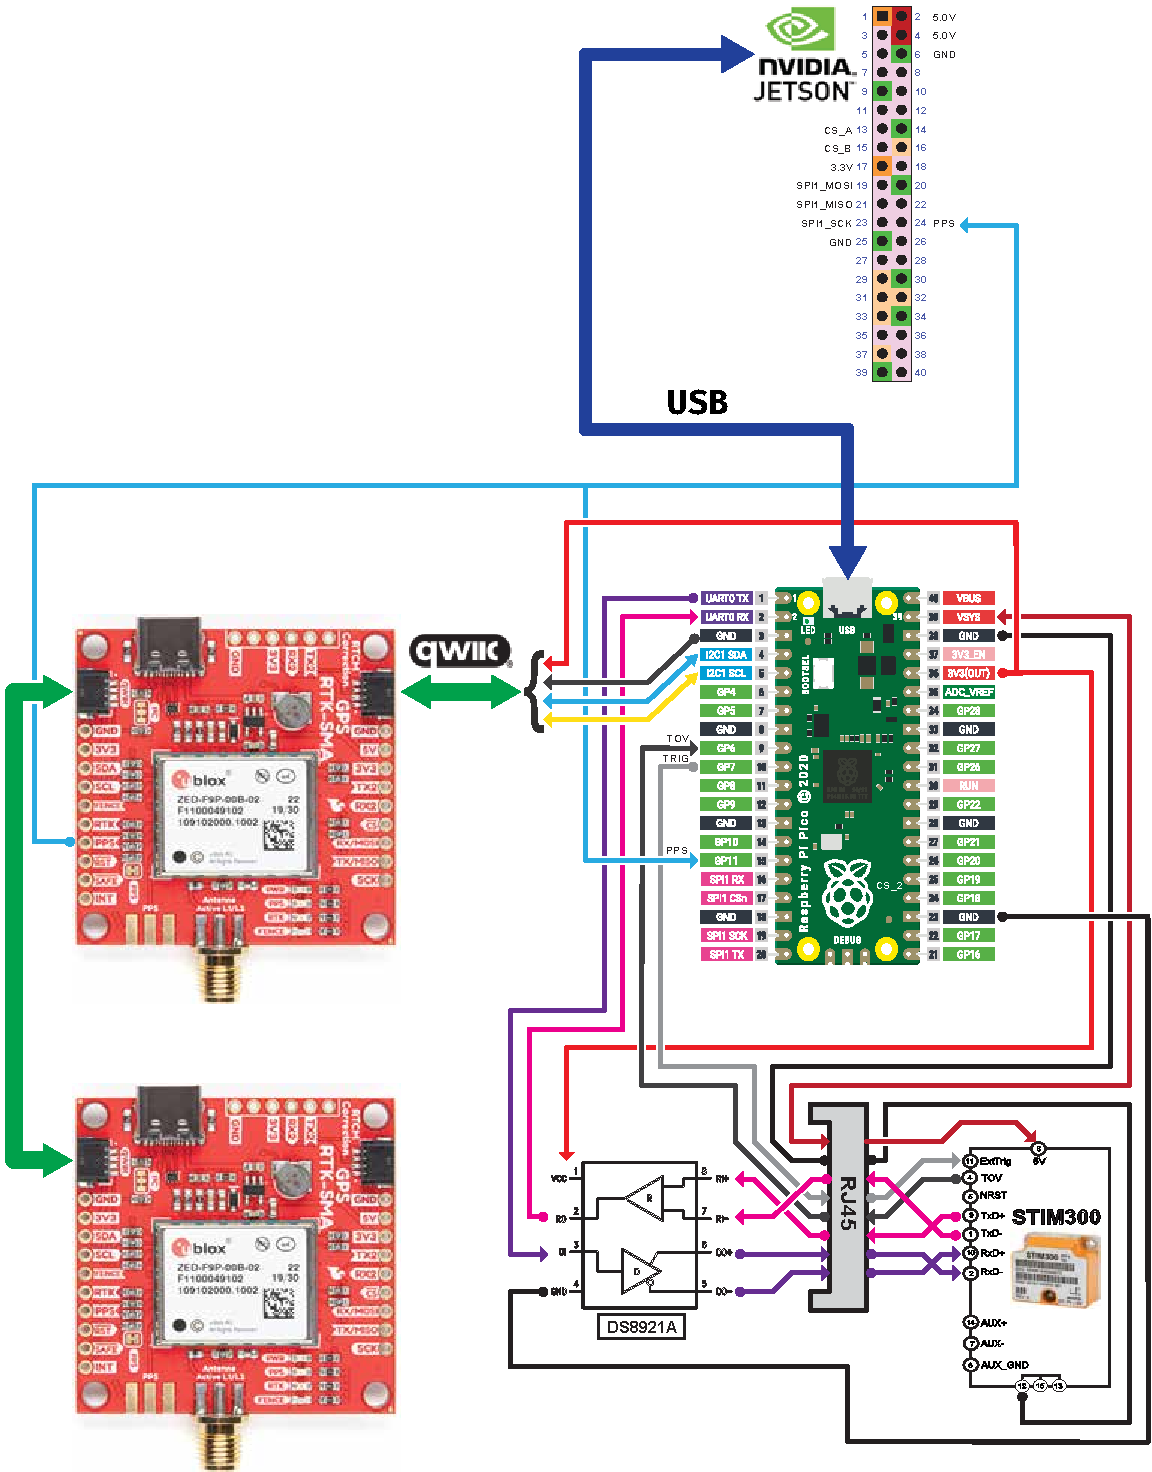
\includegraphics[width=\textwidth]{figures/navbox/navbox_usb.pdf}
    \caption{Scematics of the new \gls{navbox} interface comparet to Figure 27 of the \preproject}
    \label{fig:navbox_usb}
\end{figure}

\subsection{Improved Workflow}

To enhance the development workflow for the \gls{pico}, several improvements have been implemented.
Firstly, by configuring the \gls{cmake} file and setting the \code{PICO_STDIO_USB_RESET_MAGIC_BAUD_RATE} to $1200$ in the \gls{cmake} file, it is now possible to enter the boot mode of the \gls{pico} without the need for manual intervention by pressing the \code{bootsel} button and reconnecting it \cite{hermannswAnswerSettingUsb2021}.

Moreover, a minimal \py server has been created to make it easier to flash the \gls{pico} and communicate with it over \gls{usb} from within a \gls{docker} environment.
The server serves two primary purposes.
Firstly, it triggers the boot mode and initiates the flashing of the \gls{pico} whenever compiled code is received.
Secondly, once the \gls{pico} has been successfully flashed, the server establishes a serial connection over \gls{usb} and facilitates the bidirectional exchange of input and output data with connected clients.
This functionality is particularly valuable during code development within a container on a Windows machine, as the process of forwarding USB connections is intricate due to the \gls{pico} disconnection whenever it enters boot mode.


\subsection{Raspberry Pi Pico USB speed}

The initial selection of \gls{spi} as the communication interface was driven by the objective of enabling direct communication with the \gls{pico}, as well as both \glspl{f9p}, over a shared interface at high speeds \footnote{In this context, "high speeds" refers to transfer rates exceeding $1Mb/s$.
    Note the lowercase "b" for bit as opposed to the uppercase "B" for byte.}, as discussed in Section 4.2 of the \preproject.
This need for high speed arises because the \gls{stim} alone can generate data at a maximum frequency of $2kHz$, resulting in potential data transfer rates of up to $124kB/s$ \cite[34]{safranSTIM300Datasheet}.

Initially, there was uncertainty regarding whether the \gls{pico} could meet the requirement for high-speed communication over \gls{usb}, as the default example code for \gls{usb} communication using \code{printf} achieved only around $11kB/s$ \cite[usb/device]{RaspberryPiPico2023}.
Attempts to improve the speed by modifying the baud rate or using alternative functions such as \code{putc} or \code{puts} did not yield any improvements, which corresponds to inforamtion on the forum \cite{hippyAnswerSettingUsb2021}.
While the \gls{pico} supports \gls{usb} 1.1 and is capable of higher speeds, initial indications from various forum posts suggested that achieving those speeds would require custom-written \gls{tinyusb} drivers \cite[usb/device]{RaspberryPiPico2023}.

Fortunately, after extensive tinkering, it was serendipitously discovered that using \code{fwrite} to write to \code{stdout} without flushing the buffer until it was full resulted in speeds above $600kB/s$.
This speed is more than sufficient for data transfer from the \gls{stim} and both \glspl{f9p}.
The improved speed was attributed to transferring data in larger chunks of $4096$ bytes at a time, as opposed to smaller chunks.





